\documentclass[emulatestandardclasses]{scrartcl}
\usepackage{graphicx}
\usepackage{color}
\usepackage[dvipsnames]{xcolor}
\usepackage[ngerman]{babel}
\usepackage{hyperref}
\usepackage{fullpage}
\usepackage{calc} 
\usepackage{enumitem}
\usepackage{titlesec}
\newcommand{\todo}[1]{\textcolor{red}{TODO: #1}\PackageWarning{TODO:}{#1!}}
\date{\vspace{-3ex}}
\begin{document}

\title{
	\includegraphics*[width=0.75\textwidth]{images/hu_logo.png}\\
	\vspace{24pt}
	Wittgenstein:\\Tractatus Logico-Philosophicus}
\subtitle{Proseminar WS 16/17\\
          Dr. Jasper Liptow\\
          Philosophisches Institut I \\ 
          Humboldt Universit"at zu Berlin}
\author{Lennard Wolf\\
        \small{\href{mailto:lennard.wolf@student.hu-berlin.de}{lennard.wolf@student.hu-berlin.de}}}
\maketitle
\begin{abstract}

In seinem Tractatus logico-philosophicus (1921) pr"asentiert Ludwig Wittgenstein in atemberaubend dichter Form "Uberlegungen zum Wesen der Sprache, der Logik, der Welt und nicht zuletzt der Philosophie selbst. Seine Charakterisierung des Tractatus im Vorwort lautet kurz: \emph{Das Buch behandelt die philosophischen Probleme und zeigt – wie ich glaube – dass die Fragestellung dieser Probleme auf dem Missverst"andnis der Logik unserer Sprache beruht. Man k"onnte den ganzen Sinn des Buches etwa in die Worte fassen: Was sich "uberhaupt sagen l"asst, l"asst sich klar sagen; und wovon man nicht reden kann, dar"uber muss man schweigen.} Diese Zeilen deuten bereits an, warum der Tractatus einen der entscheidenden Schritte auf dem Weg zu einer inhaltlichen und methodischen Orientierung der Philosophie an der Sprache darstellt, wie sie die Philosophie des 20. Jahrhunderts gepr"agt hat (linguistic turn). 
Im Seminar wollen wir zum einen versuchen, den Gedankengang des Tractatus anhand einer genauen Lekt"ure zu rekonstruieren, und gucken, welche der Schmuckst"ucke aus dieser \emph{jewel box of insights} (wie der amerikanische Philosoph Wilfrid Sellars den Tractatus einmal nennt) bis heute ihren Glanz bewahrt haben.


\end{abstract}
\newpage

\tableofcontents
\newpage


\section{Einf"uhrende Sitzung\\(31.10.16)}

\textbf{Zu lesen:} 

\emph{Wittgenstein's Tractatus logico-philosophicus: A Reader's Guide} von Roger White

Selbst gefunden: 
\emph{Sprache und Wirklichkeit in Wittgensteins Tractatus} von Rolf-Albert Dietrich | \url{https://books.google.no/books?id=mwe1KLQM3bYC}

\subsection{Kontext}

In einer Liste seiner Einfl"usse war Schopenhauer der einzige Philosoph, den Wittgenstein auff"uhrte. Am wichtigsten waren jedoch Frege und Russell und deren Versuche zum Beweis des Logizismus.

\begin{description}[leftmargin=!,labelwidth=\widthof{\bfseries 2}]
  \item[Frege] War Vertreter des \emph{Logizismus} und verfolte daher das Ziel zu zeigen, dass die Axiome der Arithmetik sich aus den Axiomen der Logik herleiten lassen. Er entwickelte in seiner \emph{Begriffsschrift} die Pr"adikatenlogik erster Stufe. In seinem Buch \emph{Die Grundlagen der Arithmetik}, welches die Frage `\emph{Was sind Zahlen?}' thematisiert, stellt er das \emph{Kontextprinzip} vor, demnach Begriffe nur im Zusammenhang eines Satzes etwas bedeuten. So erh"alt etwa der Begriff `Stein' erst eine Bedeutung, wenn er im Elementarsatz `$x$ ist ein Stein' auftritt. In \emph{Grundgesetze der Arithmetik} wollte er den Logizismus voll implementieren, doch die Einf"uhrung der Mengentheorie als Axiom der Logik produzierte ein Paradox (\emph{Russelsche Antinomie}), welches von Russell erkannt wurde (z.B. Die Menge er Mengen, die sich nicht selbst beinhalten).
  \item[Russell] Selber Logizist, versuchte er mit seinem Freund Whitehead das System von Frege in der \emph{Principia Mathematica} weiterzuf"uhren und dabei das oben genannte Paradox zu vermeiden. Dazu schw"achte er das Axiom der Menge ab indem er Typen einf"uhrte. Eine Menge eines niederen Typus konnte somit keine Menge des selben oder h"oheren Typen enthalten. Durch dieses abgeschw"achte Axiom konnte aber die Arithmetik nicht mehr hergeleitet werden, weshalb Russell noch drei weitere Axiome einf"uhren musste.
  \item[Wittgensteins Einw"ande] Wittgenstein empfand die neu eingef"uhrten Axiome als k"unstlich und fragte sich, woher wir wissen k"onnen, dass sie Axiome sind. Entsprechend lassen sich folgende Fragen als Ausgangspunkt für den \emph{Tractatus} sehen: \textbf{(1)} \emph{Was l"asst sich von Russells Typentheorie halten?} und \textbf{(2)} \emph{Was l"asst sich "uber eine logische Wahrheit sagen?}. Zu letzterer Frage liesse sich sagen, dass eine logische Wahrheit \emph{notwendig} ist und \emph{a priori} erkennbar ist.
\end{description}

\subsection{Vorwort}

\emph{Das Buch will also dem Denken eine Grenze ziehen, oder vielmehr --	
 nicht dem Denken, sondern dem Ausdruck der Gedanken: Denn um dem Denken eine Grenze zu ziehen, m"ußten wir beide Seiten dieser Grenze denken k"onnen.} Wittgensteins Hauptanliegen ist es, die Philosophie von Unsinn und Verwirrung zu bereinigen, denn \emph{[d]ie meisten S"atze und Fragen, welche "uber philosophische Dinge geschrieben worden sind, sind nicht falsch, sondern unsinnig. Wir k"onnen daher Fragen dieser Art "uberhaupt nicht beantworten, sondern nur ihre Unsinnigkeit feststellen. Die meisten Fragen und S"atze der Philosophen beruhen darauf, dass wir unsere Sprachlogik nicht verstehen.} (4.003)

Die Grenzziehung in der Sprache wird die Grenzziehung zwischen \emph{sinnvollen}, \emph{sinnlosen} und \emph{unsinnigen} S"atzen sein.

\subsection{Die S"atze der ersten Gliederungsebene}
\begin{description}[leftmargin=!,labelwidth=\widthof{\bfseries 12}]
  \item[1] Die Welt ist alles, was der Fall ist.
  \item[2] Was der Fall ist, die Tatsache, ist das Bestehen von Sachverhalten.
  \item[3] Das logische Bild der Tatsachen ist der Gedanke.
  \item[4] Der Gedanke ist der sinnvolle Satz.
  \item[5] Der Satz ist eine Wahrheitsfunktion der Elementars"atze.\\
(Der Elementarsatz ist eine Wahrheitsfunktion seiner selbst.)
  \item[6] Die allgemeine Form der Wahrheitsfunktion ist: $[~\bar{p},~\bar{\xi},~N(\bar{\xi})~]$.\\
Dies ist die allgemeine Form des Satzes.
  \item[7] Wovon man nicht sprechen kann, dar"uber muss man schweigen.
\end{description}

\section{Gegenstand, Sachverhalt, Tatsache: 1 bis 2.063\\(07.11.16)}
\subsection{Lekt"urenotizen}
\subsubsection{Gedanken und Fragen}
\textbf{Gedanken}

Wittgenstein scheint in diesem Abschnitt zum einen eine terminologische Grundlage f"ur den Rest des Textes legen zu wollen, zum anderen werden aber auch schon gewissen ontologische Aussagen getroffen, zum Beispiel durch \emph{Die Welt ist die Gesamtheit der Tatsachen, nicht der Dinge.} (1.1). Ich stelle mir die nun folgende Struktur des Textes so vor, dass erst eine Ontologie entworfen wird und dann gezeigt wird, wie die Sprache (und damit das Denken?) mit der in dieser Ontologie entworfenen `Welt' in Beziehung steht. \newline
\\
\textbf{Fragen}

\begin{itemize}
  \item \emph{Eines kann der Fall sein oder nicht der Fall sein und alles "ubrige bleibt gleich} (1.21) | Soll das hei\ss en, dass Tatsachen voneinander unabh"angig sind? $\rightarrow$ steht in (2.061), aber was hei\ss t das? Wie spielt Zeit/Kausalit"at da rein?
  \item \emph{Die Substanz der Welt besteht unabh"angig von dem, was der Fall ist.} (2.024) Hei\ss t das, dass ohne eine Konfiguration die Substanz ein formloser `Blob' ist?
  \item Unterschied Welt und Wirklichkeit? Welt hat Substanz, Wirklichkeit ist nur eine `Wahrheitstafel'? 
\end{itemize}

\vspace{10pt}
\subsubsection{Neue Begriffe}

\begin{description}[leftmargin=!,labelwidth=\widthof{\bfseries Konfiguration}]
  \item[Welt] \emph{Alles} was der Fall ist. Die Gesamtheit \emph{aller} Tatsachen, d.h.  bestehenden Sachverhalte. [\emph{world}]
  \item[Tatsache] Das Bestehen (das \emph{Wahrsein}) von Sachverhalten. (\emph{Was der Fall ist}). Befinden sich im logischen Raum und sind immer wahr. [\emph{fact}]
  \item[Gegenstand] Ein einfaches Ding das nicht teilbar ist. $\rightarrow$ Auch \emph{Ding} genannt. | Um ihn zu \emph{kennen}, muss ich alle seine internen Eigenschaften kennen, d.h. auch s"amtliche M"oglichkeiten seines Vorkommens in Sachverhalten (diese liegen in seiner Natur). | K"onnen nur im Kontext von Sachverhalten vorkommen. | Identit"at ist keine Relation zwischen Gegenst"anden. [\emph{thing}, \emph{object}]
  \item[Sachverhalt] Eine Verbindung von Gegenst"anden. Sachverhalte k"onnen wahr und nicht wahr sein und sind voneinander unabh"angig. [\emph{atomic fact}, {state of affairs}]
  \item[Sachlage] Ein Komplex aus Sachverhalten.
  \item[Struktur] \emph{Die Art und Weise, wie die Gegenst"ande im Sachverhalt zusammenh"angen, ist die Struktur des Sachverhaltes.} (2.032)
  \item[Form des ??] \emph{Die Form} \emph{ist die M"oglichkeit der Struktur.} (2.033)  \item[Form des Gegenstands] \emph{Die Form} ist \emph{die M"oglichkeit seines Vorkommens in Sachverhalten}. (2.0141)
  \item[Substanz] Die Substanz der Welt ist gebildet durch die (unteilbaren) Gegenst"ande. Sie besteht unabh"angig von dem, was der Fall ist. (s. 2.024) [\emph{substance}]
  \item[Konfiguration] Die Konfiguration der Gegenst"ande bildet den Sachverhalt. Die ist das Wechselnde, Unbest"andige (im Gegensatz zu den Gegenst"anden).
  \item[Wirklichkeit] \emph{Das Bestehen und Nichtbestehen von Sachverhalten ist die Wirklichkeit.} (2.06) | \emph{Sind alle Gegenst"ande gegeben, so sind damit auch alle m"oglichen Sachverhalte gegeben.} (2.0124) | \emph{Die gesamte Wirklichkeit ist die Welt.} (2.063) {\color{red}(Was w"are halbe Wirklichkeit?)} [\emph{reality}]
\end{description}



\subsection{Sitzung}

\begin{itemize}
  \item Tatsachen sind immer in Form von S"atzen anzutreffen, w"ahrend Gegenst"ande singul"are Terme sind. 
  \item `Beispielwelt':\\\emph{Dinge}: $a, b, F, G$\\\emph{Sachverhalte}: $a$ ist $F$, $a$ ist nicht $F$,  $a$ ist $G$, $b$ ist $G$, $b$ ist nicht $F$\\\emph{Tatsachen}:  $a$ ist $F$ und $G$, $b$ ist $G$
  \item Alle letzten Elemente, in die die Welt zerf"allt, sind Tatsachen.
  \item Wir k"onnen sehr viel weniger sagen als wir denken.
  \item Sachverhalte + Logik = Tatsachen
  \item Q: \emph{Wie} atomar sind denn die Gegenst"ande? Ist ein Tisch ein Gegenstand?\\A: Ein Tisch ist ein \emph{Komplex}, aber es scheint von der Betrachtungs-/Abstraktionsebene abzuh"angen. Wittgenstein l"asst das sehr weit offen f"ur Interpretation.
  \item Q: Wann ist etwas im logischen Raum?\\A: Wenn es in logischen Beziehungen stehen kann (Die Sonne kann nicht im Widerspruch zu etwas stehen).
\end{itemize}

\section{Tatsache und Bild: 2.1 bis 3.01\\(14.11.16)}


\subsection{Lekt"ure}
\textbf{Gedanken zum Text}

\begin{figure}[h]
	\centering
	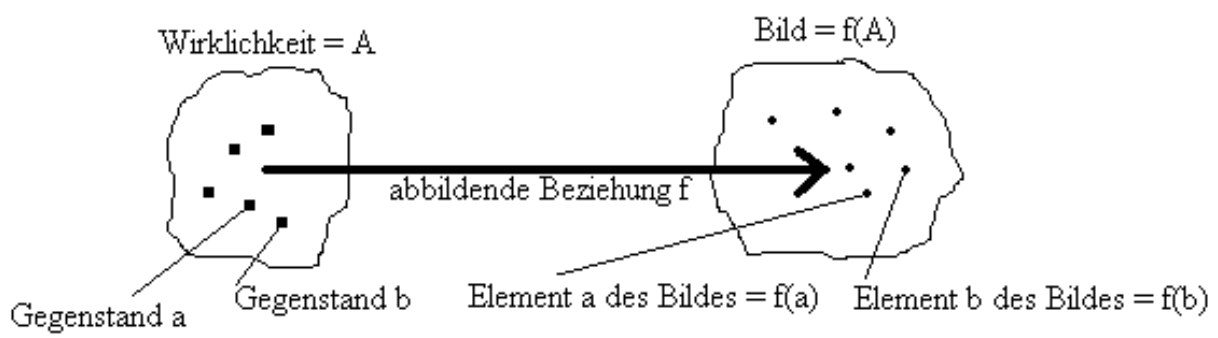
\includegraphics[width=0.7\textwidth]{images/tractatus/bild}
	\caption{Grafische Verdeutlichung des Bildbegriffs. | Quelle: \emph{Wittgensteins Bild}
von Klaus Reitberger (\url{https://klausreitberger.files.wordpress.com/2008/08/wittgensteins-bild.pdf})}
	\label{fig:bild}
\end{figure}

Abbildung \ref{fig:bild} hilft zu verdeutlichen, was unter der \emph{Form der Abbildung} zu verstehen ist: Die Art und Weise, wie sich das Element $b$ zum Element $a$ des Bildes verh"alt (und auch zu allen anderen Elementen des Bildes), nennt Wittgenstein die Struktur des Bildes. Und die M"oglichkeit, dass sich, die den Bildelementen entsprechenden Gegenst"ande (oder Dinge) $a$ und $b$ genau so zueinander verhalten, wie ihre Bilder $f(a)$ und $f(b)$, nennt Wittgenstein die \emph{Form der Abbildung}.

Tatsachen sind nicht wahr oder falsch, sondern \emph{der Fall}. Nur \emph{Aussagen "uber} Tatsachen sind wahr oder falsch.

\vspace{10pt}
\noindent \textbf{Neue Begriffe}

\begin{description}[leftmargin=!,labelwidth=\widthof{\bfseries Form der Abbildun}]
  \item[Bild] Modell der Wirklichkeit (vgl. 2.12). Es stellt die Sachlage im logischen Raum, das Bestehen und Nichtbestehen von Sachverhalten vor (vgl. 2.11). Den Gegenst"anden entsprechen im Bilde die Elemente des Bildes (vgl. 2.13), sowie die Elemente des Bildes im Bild die Gegenstände vertreten (vgl. 2.131). | Um die Wirklichkeit abbilden zu k"onnen ben"otigt das Bild die logische Form $\rightarrow$ Jedes Bild ist \emph{auch} ein logisches. (2.182) | Bild \emph{stellt} Sachverhalt \emph{dar}. Bild \emph{bildet} Tatsache \emph{ab}.
  \item[Element des Bildes] Entsprechung eines Gegenstandes im Bild (vgl. 2.13). Genauer: \emph{Vertretung} des Gegenstands.
  \item[Struktur des Bildes] Der \emph{Zusammenhang der Elemente des Bildes}. (vgl. 2.15) | Das Verh"altnis $f(a)$ zu $f(b)$
  \item[Form der Abbildung] \emph{[D]ie M"oglichkeit, da\ss~sich die Dinge so zu einander verhalten, wie die Elemente des Bildes.} (2.151) | Die M"oglichkeit, dass `Verh"altnis $a$ zu $b$' $=$ `Verh"altnis $f(a)$ zu $f(b)$'. $\rightarrow$ Die Form der Abbildung ist die M"oglichkeit der Struktur des Bildes. (vgl. 2.15) | Sie ist eine `Eigenschaft' des Bildes.
  \item[Log. Atomismus] Ansicht, dass Realit"at auf der niedrigsten ebene in unabh"angige `Etwasse' zerf"allt.
  \item[Sprache] Ist bildhaft.
\end{description}


\subsection{Hausaufgaben}

\begin{enumerate}
  \item {\color{NavyBlue}"Uber Argumentation nachdenken, warum es Gegenst"ande geben muss. (2.02 bis 2.023)}\\
{\color{ForestGreen} Aussagen im logischen Raum h"atten ohne die Substanz der Welt keinen Bezugspunkt. Da eine Aussage "uber einen Komplex, um Sinn zu haben, vorraussetzt, dass sie in Aussagen "uber die Bestandteile des Komplexes und seine Beschreibung zerlegt werden kann (2.0201), w"urde bei der Nichtexistenz von Gegenst"anden aus jeder Aussage unendlich lange regressive Aussagen ohne Bezugspunkte als die n"achste Zerteilungsebene werden. Dadurch w"are kein (brauchbares) Bild der Welt entwerfbar. Ob ein Satz wahr oder falsch ist w"are dann nur durch Bezug auf andere S"atzen begr"undbar. So w"aren Wahrheitsurteile nur regressiv und spekulativ.}
  \item {\color{NavyBlue}Erl"autern sie Wittgensteins Gedanken, dass ein Bild kein Gegenstand sondern eine Tatsache ist.}\\
{\color{ForestGreen} Ein Bild kann kein Gegenstand sein, weil es (u.a.) die logische Form hat. Ein Bild muss zum einen mit der Tatsache die Form gemein haben, um sie abbilden zu k"onnen, und es muss `der Fall sein', damit es `gedacht' werden kann. Wenn es nicht der Fall w"are, w"ürde man nicht mit ihm interagieren.}
  \item {\color{NavyBlue} Warum muss ein Bild mit dem Abgebildeten die Form der Abbildung gemein haben?}\\
{\color{ForestGreen}Wenn dies so nicht w"are, dann w"are es nicht m"oglich, einen Isomorphismus zu bilden. Ohne einen solchen w"are das Bild nicht verst"andlich.}
  \item {\color{NavyBlue}Warum l"asst sich die Form der Abbildung nicht abbilden?}\\
{\color{ForestGreen} Weil es sich um komplett unterschiedliche Kategorien handelt. Die Form ist nur die M"oglichkeit der Struktur, sie hat keine Substanz. Ein Bild \emph{weist die Form der Abbildung auf}. (2.172)}

\end{enumerate}



\begin{figure}[h]
	\centering
	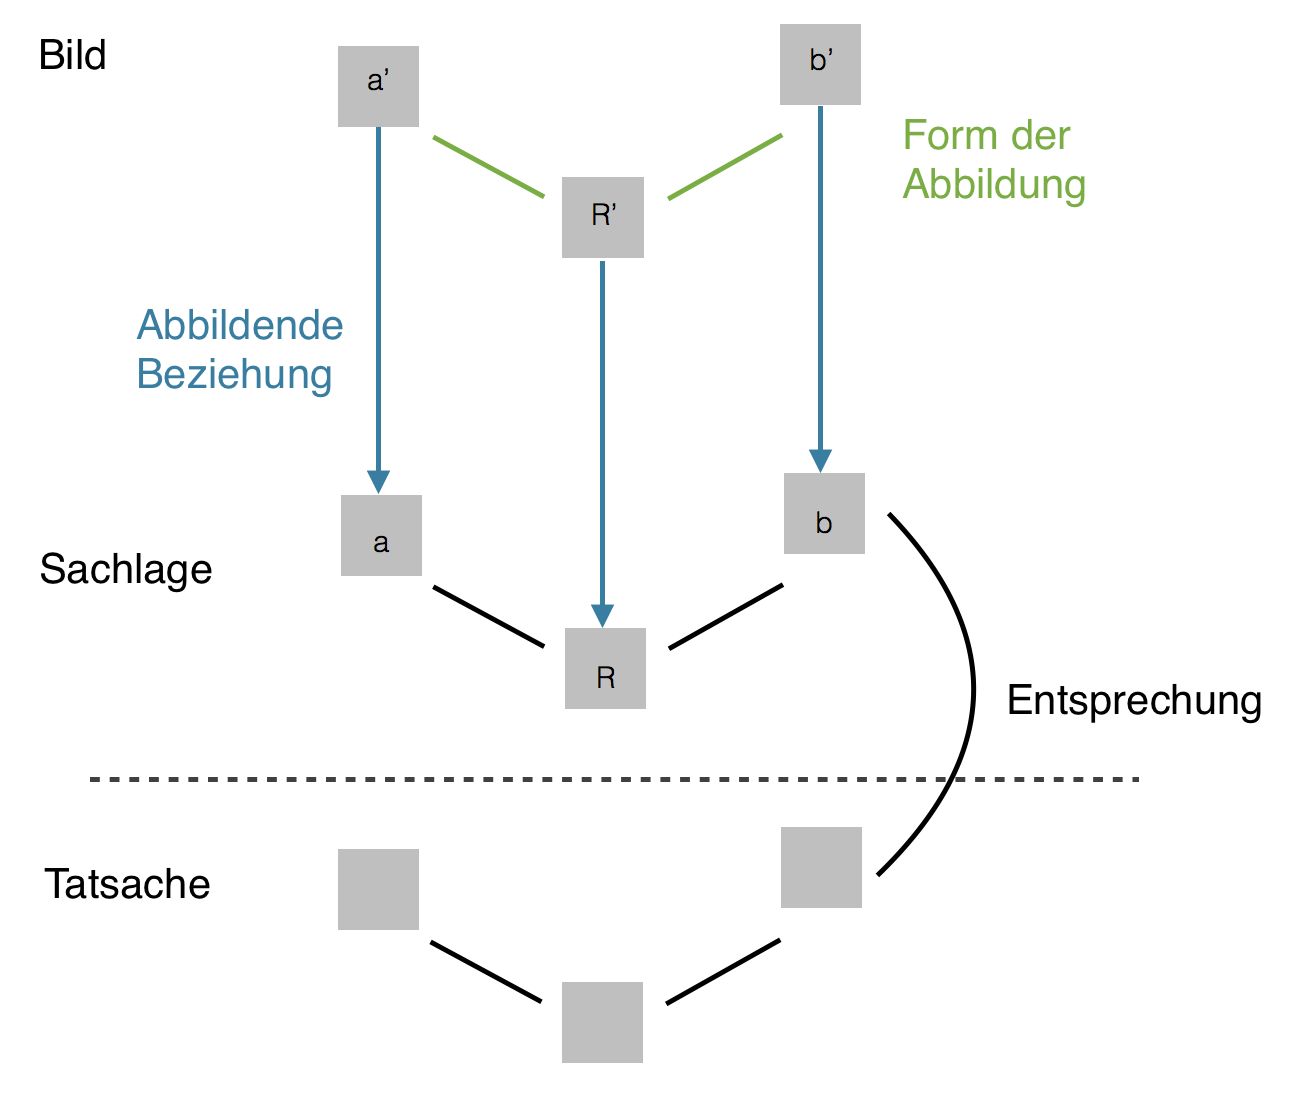
\includegraphics[width=0.6\textwidth]{images/tractatus/bilder.png}
	\caption{Die Zusammenh"ange von Bildern, Sachlagen und Tatsachen}
	\label{fig:bilder}
\end{figure}


\section{Satz und Name: 3 bis 3.263\\(21.11.16)}

\begin{center}
    \begin{tabular}{  l | l }
    \textbf{Wirklichkeit} & \textbf{Sprache}\\ \hline
    Gegenstand & Name \\ 
    Sachverhalt & Elementarsatz \\
    Sachlage & Satz \\
    \end{tabular}
\end{center}



\subsection{Lekt"urenotizen}

\vspace{10pt}
\subsubsection{Neue Begriffe}

\begin{description}[leftmargin=!,labelwidth=\widthof{\bfseries Satzzeichen}]
  \item[Gedanke] \emph{Das logische Bild der Tatsachen ist der Gedanke.} (3)
  \item[Satz] \emph{Im Satz dr"uckt sich der Gedanke sinnlich wahrnehmbar aus.} (3.1) | Das Satzzeichen in seiner projektiven Beziehung zur Welt. | Ein Satz kann nur sagen \emph{wie} ein Ding ist, nicht \emph{was}.
  \item[Satzzeichen] Projektion der m"oglichen Sachlage | \emph{Das Zeichen, durch welches wir den Gedanken ausdrücken, nenne ich das Satzzeichen.}
  \item[Name] Bedeutet den Gegenstand und vertritt ihn im Satz.
  \item[Urzeichen]
  \item[Anwendung]
\end{description}

\subsubsection{Fragen}

\begin{itemize}
  \item Ist ein Satzzeichen ein Bild?
  \item Interpretationsregeln zu S"atzen?
  \item Unterschied Sinn/Bedeutung?
  \item Was hei"st \emph{artikuliert}?
  \item Gibt es Logik ohne Menschen?
\end{itemize}

\subsubsection{Hausaufgaben}

\begin{enumerate}
  \item {\color{NavyBlue}Zusammenhang Satz, Satzzeichen, Bild, Inhalt des Bildes.}\\
{\color{ForestGreen} blabla}
  \item {\color{NavyBlue} Rekontruieren Sie Wittgensteins Verst"andnis des Satzes.}\\
{\color{ForestGreen} blabla}
\end{enumerate}


\section{Primat des Satzsinns: 3.3 bis 3.5\\(28.11.16)}


\subsection{Analyse eines Satzes}

Im Grunde im Sinne Russells.

\begin{center}
    \begin{tabular}{ l| l | l }
     & \textbf{Sokrates} & \textbf{ist weise.}\\ \hline
    Def/Analyse & $\exists !~x~(x$ ist $F)$ & $x$ ist $G$  \\
    Def/Analyse & $(a$ ist $F$ und $G)~\vee~(b$ ist $F$ und $G)~\vee ... \vee~(n$ ist $F$ und $G)$ 
    \end{tabular}
\end{center}

S"atze wie `$(a$ ist $F$ und $G)$' sind \emph{Elementars"atze}. Jeder (wahre) Elementarsatz bezieht sich dann auf eine elementare Tatsache/einen Sachverhalt. (`Sokrates' ist ein Alltagsname und bezieht sich auf einen Komplex. $a$ w"are ein Name f"ur einen Gegenstand und $F$ w"are eine \emph{externe} Eigenschaft.)

\subsection{Neue Begriffe}

\begin{description}[leftmargin=!,labelwidth=\widthof{\bfseries Logische Syntax}]
  \item[Kontextprinzip] (3.3)
  \item[Ausdruck] die Anzahl der Ausdr"ucke ist gleich der Zahl der Elementars"atze | Anzahl der W"orter $\neq$ Anzahl der Ausdr"ucke
  \item[Satzvariable] Der Satz `\emph{Sokrates ist weise.}' besteht aus den Satzvariablen `\emph{Sokrates ist} $X$.', bzw. `$X$(Sokrates)' und `$x$ \emph{ist weise}.', bzw. `$W(x)$' und hat damit selbst die Form `$X(x)$'. 
  \item[Logische Syntax] Die Logik ist eine \emph{Symbolsprache}. Was Sprachen wie aus der Begriffsschrift 
  \item[Name] Ist eine Satzvariable! (Beispiel: \emph{nicht} `Platon' sondern `Platon ist $X$').
  \item[Symbol] Ist ein Ausdruck. 
  \item[Zeichen] Das sinnlich wahrnehmbare am Symbol. Willk"urlich.
  \item[Definition] \emph{Definitionen sind Regeln der Übersetzung von einer Sprache in eine andere. Jede richtige Zeichensprache muss sich in jede andere nach solchen Regeln übersetzen lassen: Dies ist, was sie alle gemeinsam haben.} (3.343)
  \item[Logischer Ort] Satzzeichen und die logischen Koordinaten
\end{description}

Die Funktion bildet Ausdr"ucke auf S"atze ab.

\begin{enumerate}
  \item {\color{NavyBlue}Warum sagt Wittgenstein, dass ein Ausdruck nur im Satz Bedeutung hat?}\\
{\color{ForestGreen} Ein Ausdruck hat nur im Satz Bedeutung, weil er eine Satzvariable ist, die ohne eine Festsetzung des variablen Abschnitts, keinen Sachverhalt darstellt.}
  \item {\color{NavyBlue}Was ist der Unterschied zwischen \emph{Zeichen} und \emph{Symbol}? }\\
{\color{ForestGreen} Das Zeichen ist das sinnlich wahrgenommene und referiert ein exaktes Symbol, welches wiederum ein Ausdruck ist. (Ein Symbol kann von vielen Zeichen dargestellt werden.) (vgl. 3.32)} | Beispiel: Das Zeichen `ist' kann, abh"angig vom Kontext,  die verschiedenen Symbole `$F(a)$', `$x = y$' und `$\exists x~ x = y$' meinen. 
\end{enumerate}


\subsection{Fundamentale Verwechselungen}
%\textbf{Gedanken zum Text}\\
Zeichen mit selber \emph{oberfl"achengrammatikalischen} Form k"onnen Symbole ganz unterschiedlicher logischen Form sein! (3.23) Dadurch k"onnen in Umgangssprache Verwirrungen auftauchen! | Beispiel: Gott friert. $\rightarrow$ $F(Gott)$. \textbf{vs.} Gott existiert.  $\rightarrow$ `$\exists x~x$ ist Gott'.\\

\noindent \textbf{Daher:} So entstehen leicht die fundamentalsten Verwechselungen (deren die ganze Philosophie voll ist). (3.324) !


\section{Der Satz: 4 bis 4.0641\\(05.12.16)}

\vspace{10pt}

\subsection{Typentheorie}

\begin{description}[leftmargin=!,labelwidth=\widthof{\bfseries Typentheorie}]
  \item[Russells Paradox] Die Menge aller Mengen die sich selbst nicht enthalten. $\rightarrow$ Naive Mengentheorie nach Frege kann nicht g"ultig sein.
  \item[Typentheorie] 
\end{description}

\subsection{Neue Begriffe}

Ich kann einen Satz verstehen oohne seine logische Form zu kennen.

\begin{description}[leftmargin=!,labelwidth=\widthof{\bfseries Typentheorie}]
  \item[Sinn des Satzes] Die dargestellte Sachlage, der ausgedr"uckte Gedanke.
  \item[Sinnvoll] Der Gedanke ist der sinnvolle Satz. Bsp: "`C"asar ist eine lustige Primzahl."' (sinnvoll, aber falsch)
  \item[Unsinnig] Grammatikalisch/Syntaktisch falsch: "`Demokratien sind dunkler als gestern."'
  \item[Typentheorie] \emph{Kein Satz kann etwas über sich selbst aussagen, weil das Satzzeichen nicht in sich selbst enthalten sein kann (das ist die ganze »Theory of Types«).} $\rightarrow$ Daher ist Typentheorie falsch.
  \item[Sprache] Gesamtheit der S"atze. Verkleidet den Gedanken. 
  \item[Satz] Beschreibung/logisches Bild des Sachverhaltes. Einen Satz verstehen, heißt, wissen was der Fall ist, wenn er wahr ist. (Man kann ihn also verstehen, ohne zu wissen, ob er wahr ist.) Man versteht ihn, wenn man seine Bestandteile versteht.
\end{description}



\section{Was S"atze Darstellen k"onnen und was nicht: 4.1 bis 4.128\\(12.12.16)}

\subsection{Neue Begriffe}

\begin{description}[leftmargin=!,labelwidth=\widthof{\bfseries Sachverhalt}]
  \item[Formale Eigenschaft] Auch interne Eigenschaft. Sie \emph{zeigt} sich
  \item[Formaler Begriff] Scheinbegiffe also gar keine Begriffe, z.B. "`Gegenstand"'. bezieht sich auf die \emph{Struktur} von Sachverhalten. Es \emph{zeigt} sich, dass "`x ist ein Gegenstand"'.
  \item[Unsagbares] S"atze mit formalen Begriffen
  \item[Eigentlicher Begriff] (zeigen) 
\end{description}

\subsection{Fragen}

\begin{enumerate}
  \item {\color{NavyBlue}Unterschied Philosophie und Naturwissenschaften}\\
{\color{ForestGreen} Naturwissenschaften (Weltbeschreibung/Tatsachendarstellung) treffen Aussagen "uber die Welt Philosophie \emph{nicht}. Philosophie erl"autert (Erl"autern ist eine \emph{T"atigkeit})}
  \item {\color{NavyBlue} Wie kann es etwas geben, das sich mit S"atzen nicht sagen aber zeigen l"asst, wenn sich mit s"atzen doch die gesamte Wirklichkeit darstellen l"asst.}\\
{\color{ForestGreen} blabla}
    \item {\color{NavyBlue} Unterschied formale Eigenschaften/Relationen und formale Begriffen}\\
{\color{ForestGreen} blabla}
\end{enumerate}




\section{Satzsinn und Elementars"atze: 4.2 bis 4.53\\Der Satz als Wahrheitsfunktion der Elementars"atze: 5 bis 5.22\\(09.01.17)}

"Uberspringen: Wahrscheinlichkeit: 5.15

\vspace{10pt}
\subsection{Neue Begriffe}

\begin{description}[leftmargin=!,labelwidth=\widthof{\bfseries St}]
  \item[Logischer Atomismus] Er behauptet, dass die Analyse von gew"ohnlichen S"atzen zu einer zugrunde liegenden idealen, logischen Sprache führt, deren S"atze in einer abbildenden Beziehung zu atomaren Tatsachen (beziehungsweise Sachverhalten) stehen. 
  \item[Elementarsatz] die kleinsten sprachlichen Einheiten, welche Wahrheitswerte annehmen, das heißt nur S"atze, welche eine Relation aus $n$ "`Namen"' beinhalten und keine wahrheitsfunktionalen Operatoren (wie "`und"', "`oder"', "`nicht"') und keine Quantoren (wie "`alle"') | beziehen sich auf \emph{Elementare Sachverhalte}
  \item[Tatsache] Tatsachen sind Elementars"atze mit wahrheitsfunktionalen Operatoren
  \item[Wahrheitstafeln] Innerer Zusammenhang eines Satzes ist durch Wahrheitstafeln erkennbar | sie legen die logische Form und den Sinn eines Satzes fest
  \item[Sinnlos] Tautologie und Kontradiktion: aus diesen S"atzen folgt nichts "uber die Welt
  \item[Sinn eines Satzes]  
\end{description}

Dem und und der Folgerung und allen Junktoren entspricht nichts in der Welt, denn sie sind miteinander austauschbar
Ist die Ontologie des Tractatus kompatibel mit der Alain Badious? 

\section{5.23 bis 5.5571\\(16.01.17)}

\vspace{10pt}
\subsection{Neue Begriffe}

\begin{description}[leftmargin=!,labelwidth=\widthof{\bfseries Successive Anwendung}]
  \item[Struktur der S"atze] ...
  \item[Successive Anwendung] 
  \item[Wahrheitsfunktion] 
  \item[Wahrheitsoperation] Die Art und Weise, wie aus den Elementars"atzen die Wahrheitsfunktion entsteht. | Ein Satz ist das Resultat von Wahrheitsoperationen mit Elementas"atzen. (5.3)
  \item[Successive Anwendung] $[a, x, O'x] \rightarrow a, O'a, O'O'a, ...$, gleichzusetzen mit \emph{etc.}
\end{description}

\section{6 bis 6.241\\(16.01.17)}

\vspace{10pt}
\subsection{Neue Begriffe}

Die allgemeine Form der Wahrheitsfunktion ist: $[~\bar{p},~\bar{\xi},~N(\bar{\xi})~]$.\\

\begin{description}[leftmargin=!,labelwidth=\widthof{beliebige sdf}]
  \item[ $[~\bar{p},~\bar{\xi},~N(\bar{\xi})~]$] Allgemeine Form der Wahrheitsfunktion (Alles was sagbar ist)
  \item[$\bar{p}$] Die Menge aller Elementars"atze
  \item[$\bar{\xi}$] Eine beliebige Menge von Elementars"atzen ($\bar{\xi}~\subset~\bar{p}$)
  \item[$N(\bar{\xi})$] Successive Anwendung der Operation $N$ (Negation) auf die Elementars"atze $\bar{\xi}$
  \item[Satz der Logik] Tautologie (Gesetz der Logik), Denkvorschruft $\rightarrow$ es gibt keine selbstevidenten logischen Wahrheiten
  \item[Logik] Methode mit der wir zeigen k"onnen dass S"atze wahr sind; Die Gesamtheit aller Tautologien
\end{description}

\subsection{Fragen}

\begin{itemize}
  \item 
\end{itemize}


\newpage
\section{Anhang}

\subsection{Disclaimer}

Textausschnitte k"onnen zum Teil oder komplett aus Internetquellen direkt oder editiert "ubernommen worden sein. Daher erhebe ich in diesem Werk \emph{keinen} Anspruch auf origin"ar auktorale Arbeit. Es handelt sich \emph{ausschlie\ss lich} um eine Begleitarbeit zum Studium. Der "Ubersicht halber werden Quellenangaben innerhalb des Texts auch unterlassen. 

Sollte sich die Person, von der ein sich in diesem Text befindlichen Textst"uck urspr"unglich verfasst wurde, daran st"oren, bitte ich diese Person mich "uber die auf der Titelseite angegebene e-mail Adresse zu kontaktieren.
\subsection{Abbildungen}

\begin{figure}[h]
	\centering
	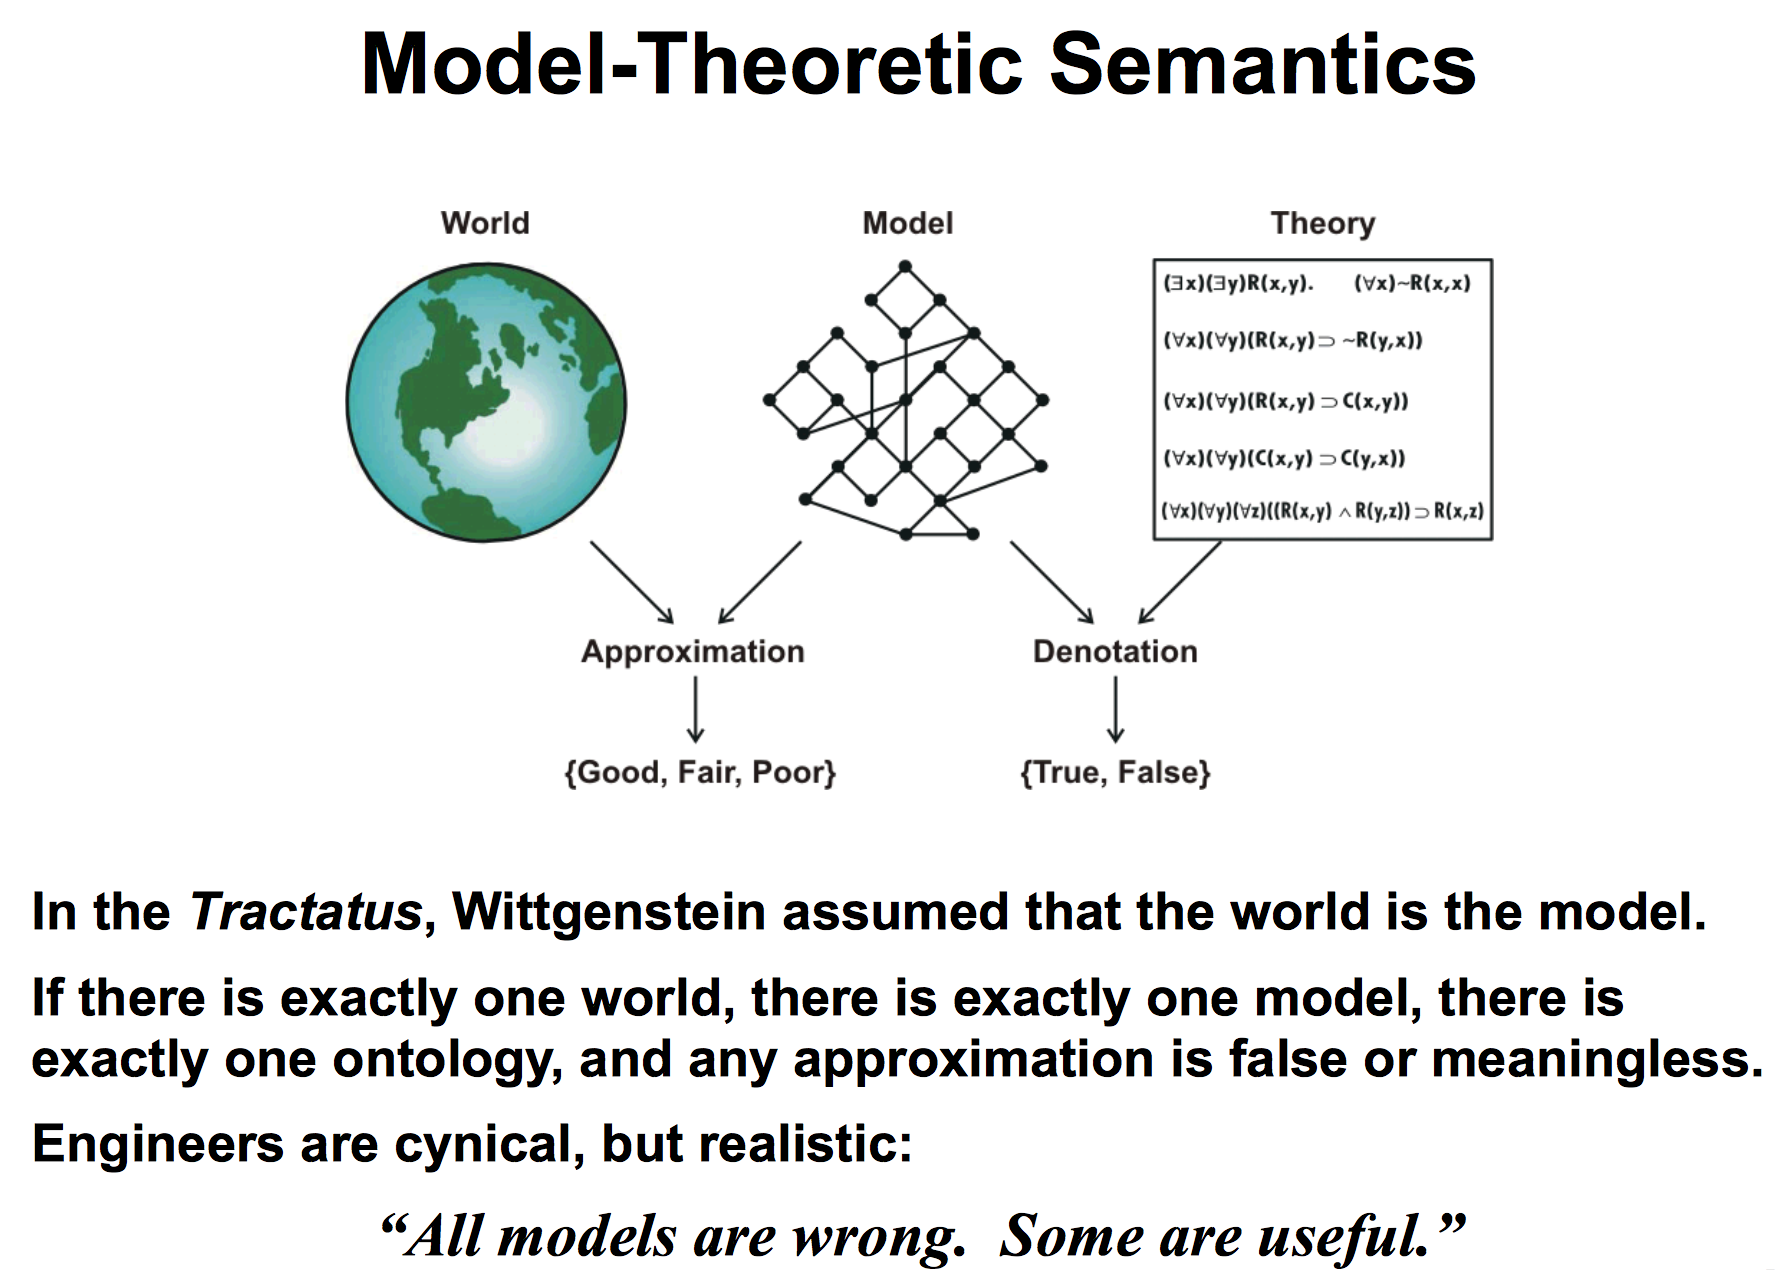
\includegraphics[width=0.6\textwidth]{images/tractatus/semantics.png}
	\caption{A Figure.}
	\label{fig:sem}
\end{figure}
\begin{figure}[h]
	\centering
	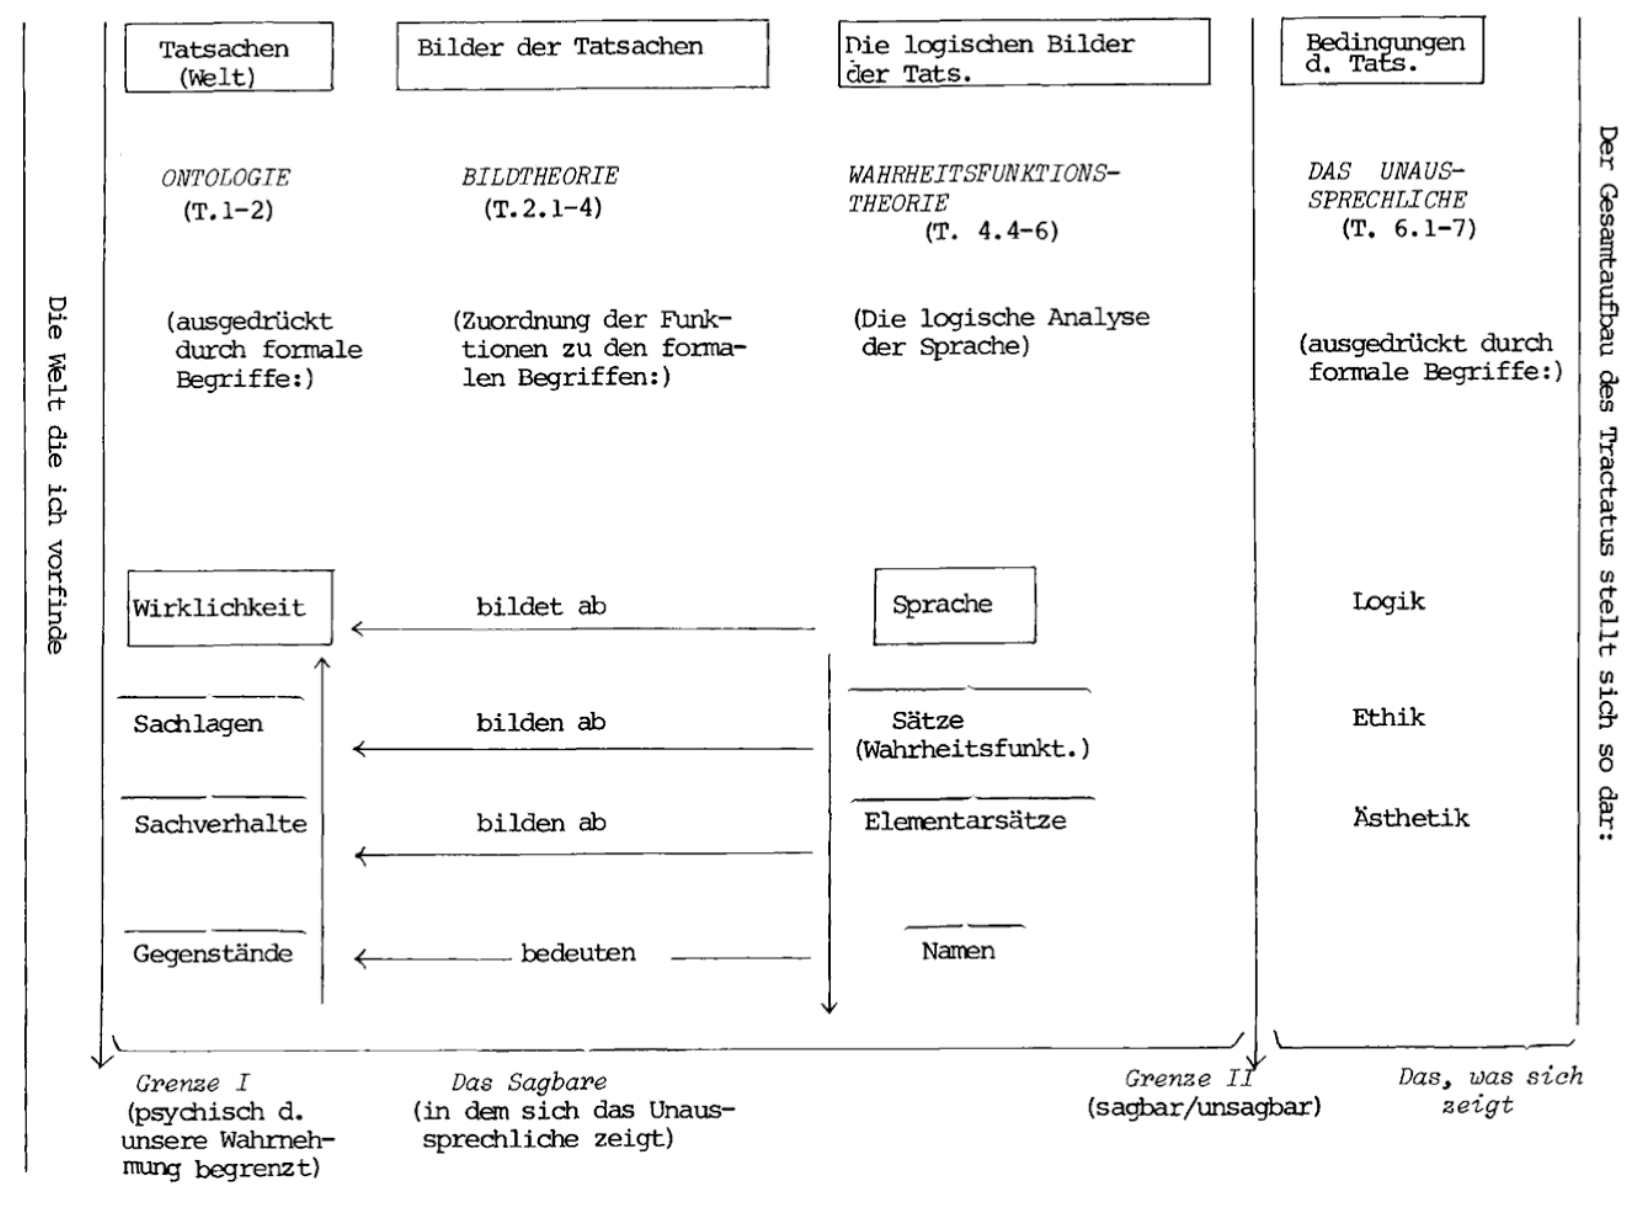
\includegraphics[width=1\textwidth]{images/tractatus/tractatus-structur.png}
	\caption{Der Gesamtaufbau des Tractatus. | Quelle: \emph{Sprache und Wirklichkeit in Wittgensteins Tractatus} von Rolf-Albert Dietrich}
	\label{fig:struct}
\end{figure}
\begin{figure}[h]
	\centering
	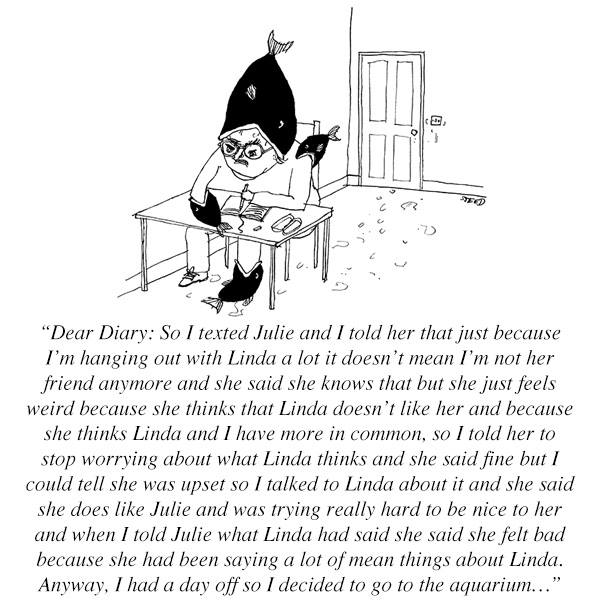
\includegraphics[width=0.6\textwidth]{images/tractatus/newyorker}
	\caption{\emph{Sinnvoll}, \emph{Sinnlos} oder \emph{Unsinnig}? | Quelle: Cartoon aus dem \emph{New Yorker} von Edward Steed}
	\label{fig:newyorker}
\end{figure}


%\newpage
%\section{"Uber den Dozenten}
%Dr. Jasper Liptow absolvierte 1996 seinen Magister an der Universit"at Hamburg, promovierte in Gie\ss en mit einer Arbeit zum Thema \emph{Gebrauchstheorien der Bedeutung} bei Prof. Martin Seel und ist Privatdozent.
%
%
%\begin{figure}[]
%	\centering
%	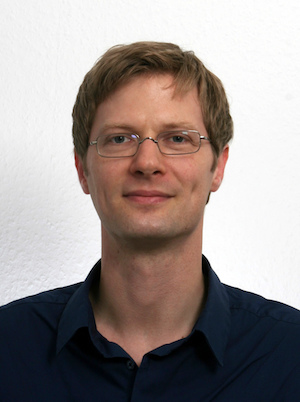
\includegraphics[width=0.32\textwidth]{images/liptow.jpg}
%	\caption{Dr. Jasper Liptow. | Quelle: \url{https://www.uni-frankfurt.de/45457854/liptow.jpg}}
%	\label{fig:liptow}
%\end{figure}
%


%\begin{figure}[h]
%	\centering
%	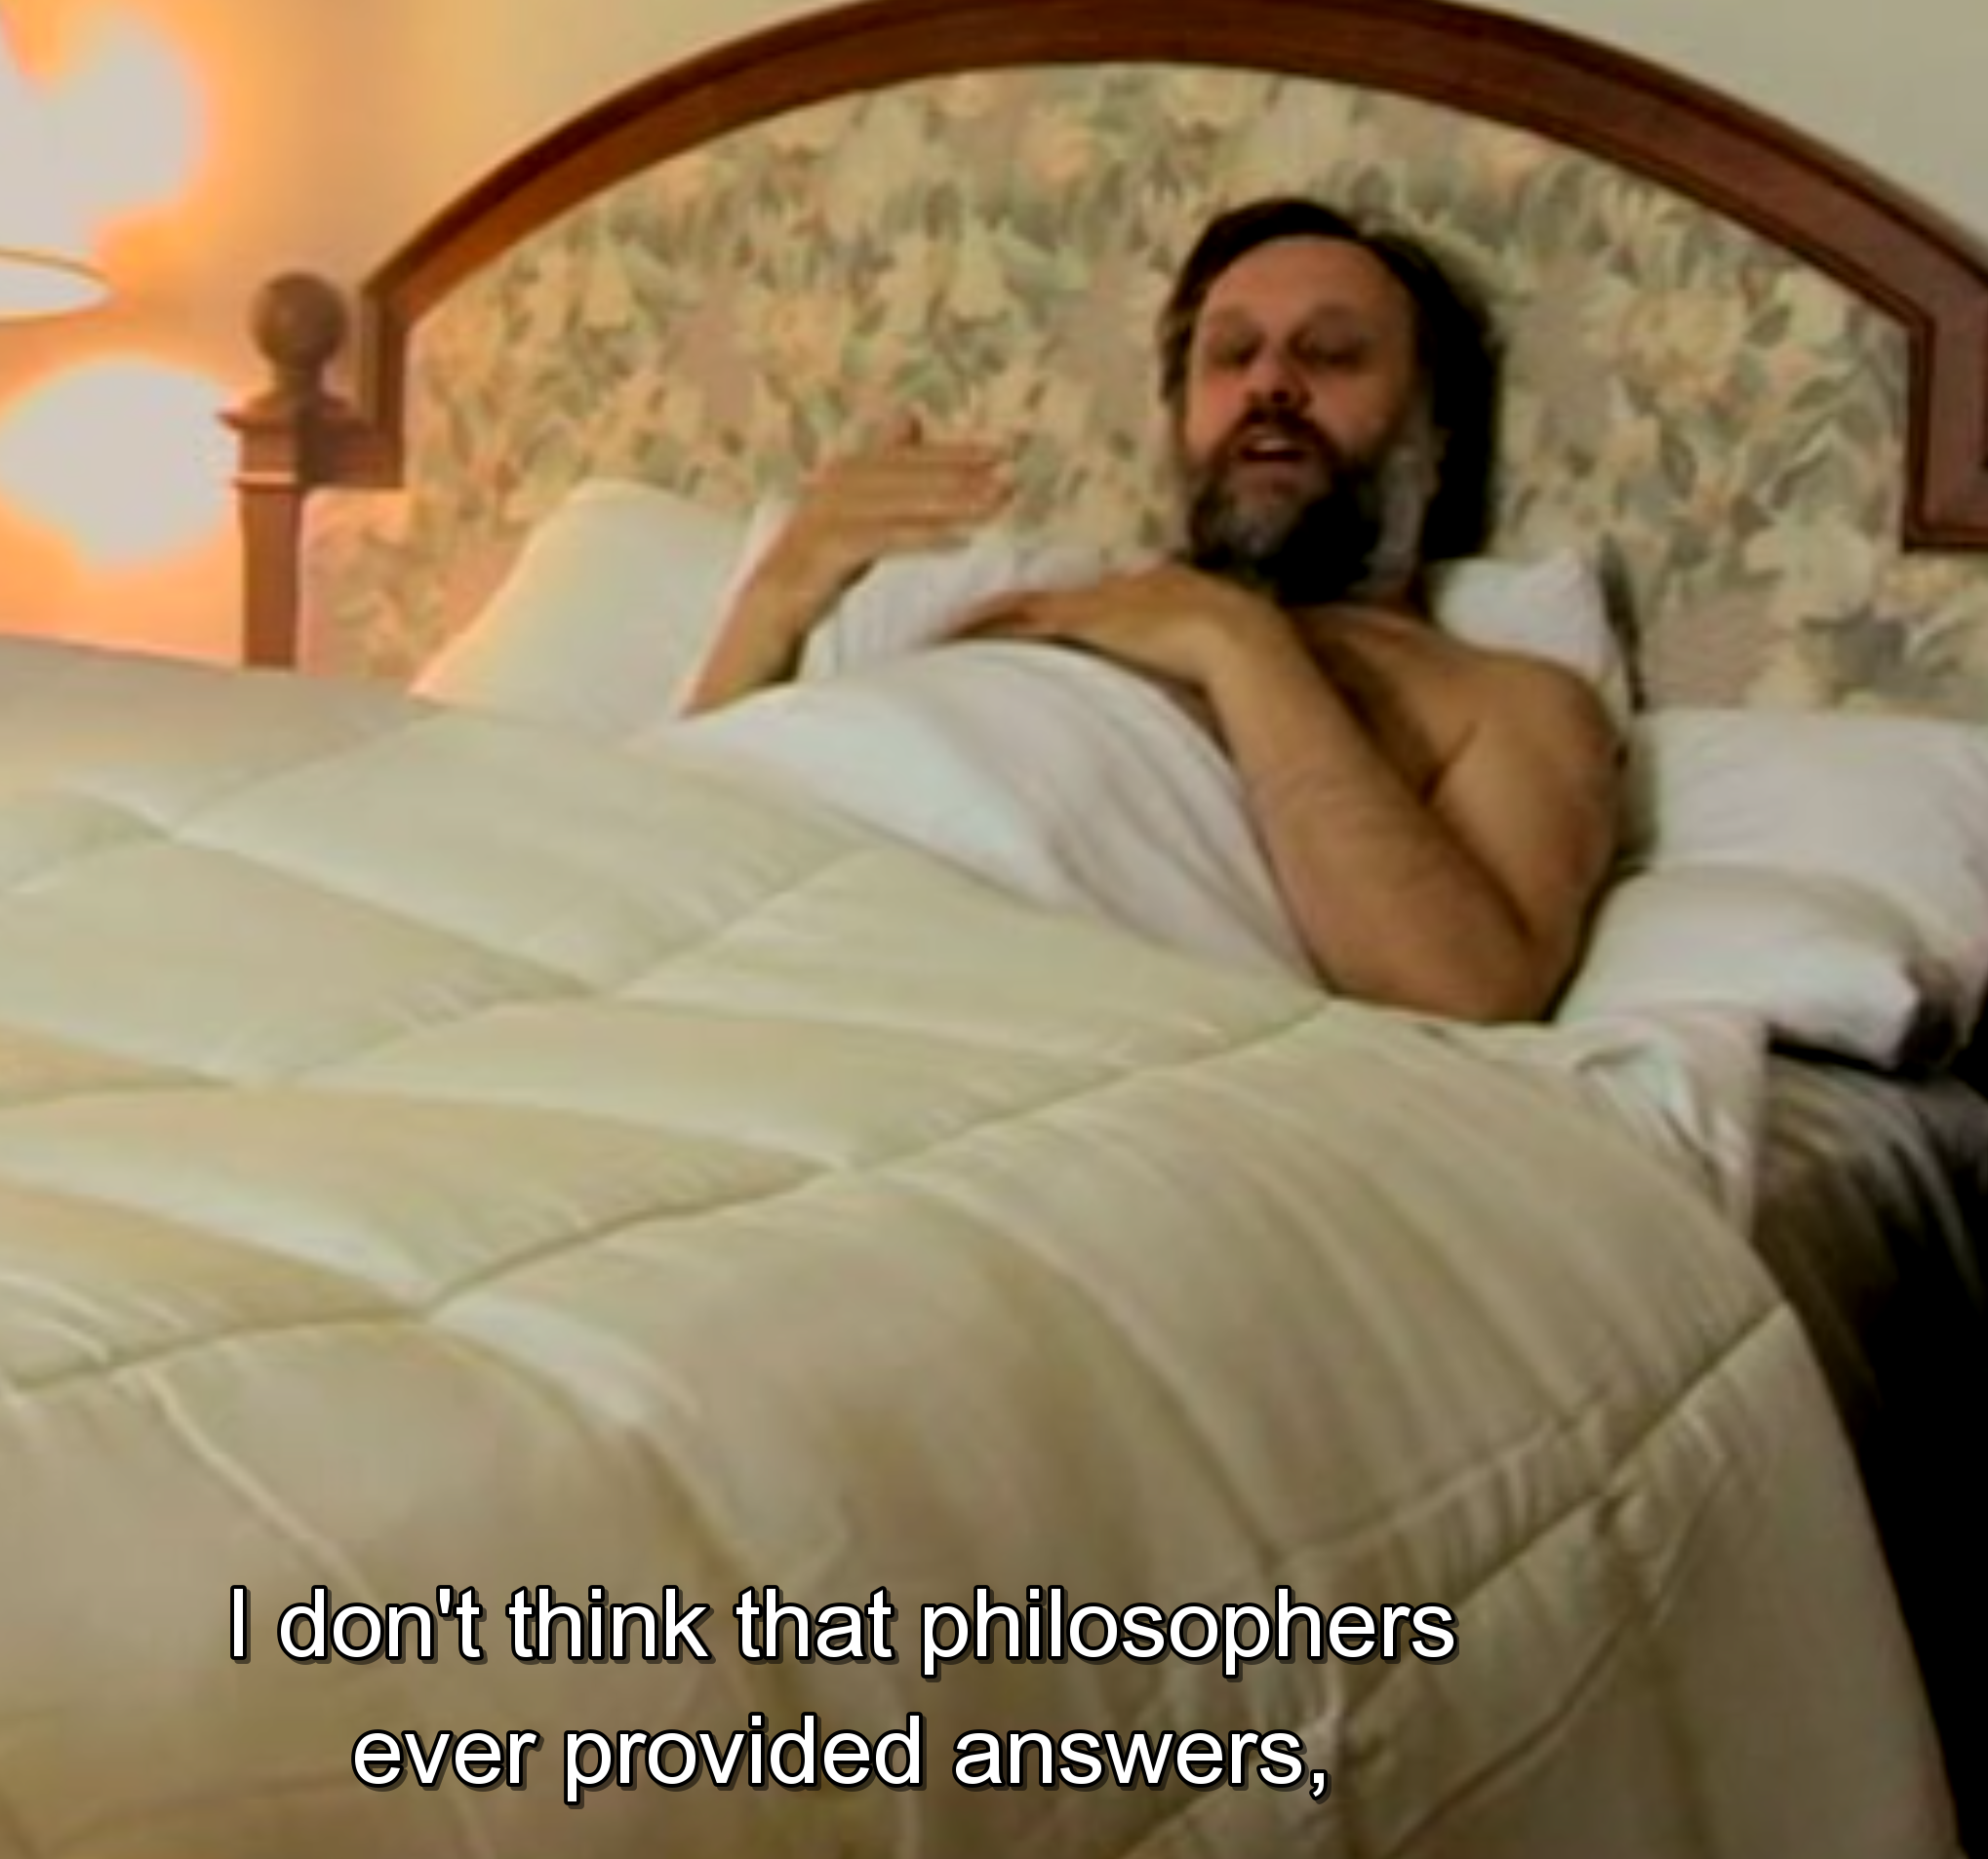
\includegraphics[width=0.5\textwidth]{images/template.png}
%	\caption{Template Bild}
%	\label{fig:template}
%\end{figure}

\end{document}
